\documentclass[11pt,a4paper]{article}
\usepackage[margin=2.2cm]{geometry}
\usepackage{amsmath,amssymb,bm}
\usepackage{booktabs,array}
\usepackage{enumitem}
\usepackage{xcolor}
\usepackage[breakable,skins]{tcolorbox}
\usepackage{tikz}
\usetikzlibrary{arrows.meta,positioning,calc,fit,shapes.geometric}
\usepackage{pgfplots}
\pgfplotsset{compat=1.18}
\usepgfplotslibrary{fillbetween}
\usepackage[colorlinks=true,linkcolor=blue!50!black,urlcolor=blue!50!black]{hyperref}
\usepackage{fancyhdr}

\definecolor{idea}{RGB}{30,90,160}
\definecolor{exam}{RGB}{20,120,70}
\definecolor{warn}{RGB}{170,60,30}

\newtcolorbox{keyidea}[1][Key idea]{breakable,before upper={\setlength{\parskip}{6pt}},colback=idea!5,colframe=idea!70!black,title={#1},fonttitle=\bfseries}
\newtcolorbox{example}[1][Worked example]{breakable,before upper={\setlength{\parskip}{6pt}},colback=exam!5,colframe=exam!70!black,title={#1},fonttitle=\bfseries}
\newtcolorbox{caution}[1][Watch out]{breakable,before upper={\setlength{\parskip}{6pt}},colback=warn!5,colframe=warn!70!black,title={#1},fonttitle=\bfseries}

\newcommand{\N}{\mathcal{N}}
\newcommand{\LL}{\mathcal{L}}

\pagestyle{fancy}
\fancyhf{}
\lhead{CSE-5025 Generative AI}
\rhead{Study Notes: GMMs and the EM Algorithm}
\cfoot{\thepage}
\setlength{\headheight}{14pt}
\setlength{\parindent}{0pt}
\setlength{\parskip}{5pt}

\begin{document}

\begin{center}
{\LARGE\bfseries Gaussian Mixture Models and the EM Algorithm}\\[6pt]
Study notes with explanations and worked numerical examples\\
CSE-5025 Generative Artificial Intelligence, MS Fall 2026, CSE, University of Dhaka\\
Based on the course handout \texttt{gmm-kmean-em-markov\_2.pdf}
\end{center}

\begin{keyidea}[How to read these notes]
The handout uses one running example: \textbf{student examination marks}. These notes follow the same sections and keep the same numbers, so you can read them side by side. Every number from the handout was recomputed and checked. Where the handout skips steps (variance sums, the log-likelihood, later EM iterations), the missing arithmetic is filled in, and extra examples are added for the limitations section. Boxes marked \emph{Worked example} contain calculations; boxes marked \emph{Watch out} flag common mistakes.
\end{keyidea}

\tableofcontents
\newpage

%======================================================================
\section{The Gaussian Distribution}
%======================================================================

A Gaussian (normal) distribution describes values clustered around a central value, the \textbf{mean}. We write $x\sim\N(\mu,\sigma^2)$ where
\begin{itemize}[nosep]
\item $\mu$: \textbf{mean}, the centre of the distribution;
\item $\sigma^2$: \textbf{variance}, how spread out the values are;
\item $\sigma$: \textbf{standard deviation}, $\sigma=\sqrt{\sigma^2}$, in the same units as $x$.
\end{itemize}
The probability density function (PDF) is
\[
\boxed{\;p(x)=\N(x\mid\mu,\sigma^2)=\frac{1}{\sqrt{2\pi\sigma^2}}\exp\!\left(-\frac{(x-\mu)^2}{2\sigma^2}\right).\;}
\]

\textbf{Reading the formula.}
\begin{itemize}[nosep]
\item $(x-\mu)^2$: squared distance from the centre. The density is largest at $x=\mu$, where the exponent is $0$.
\item Dividing by $2\sigma^2$: distance is measured \emph{relative to the spread}. Being 10 marks from the mean is far if $\sigma=5$ but close if $\sigma=20$.
\item $1/\sqrt{2\pi\sigma^2}$: normalising constant that makes the total area exactly $1$. A wider Gaussian is therefore also \emph{lower}.
\end{itemize}

\begin{center}
\begin{tabular}{@{}ll@{}}
\toprule
Feature & Explanation\\
\midrule
Symmetric & Left and right sides are mirror images about $\mu$.\\
Bell-shaped & Highest density at the mean.\\
Mean $=$ Median $=$ Mode & All three equal $\mu$.\\
Total area $=1$ & It is a probability density.\\
Continuous & $x$ can take any real value.\\
Tails & Extend forever in both directions (never exactly $0$).\\
\bottomrule
\end{tabular}
\end{center}

\begin{center}
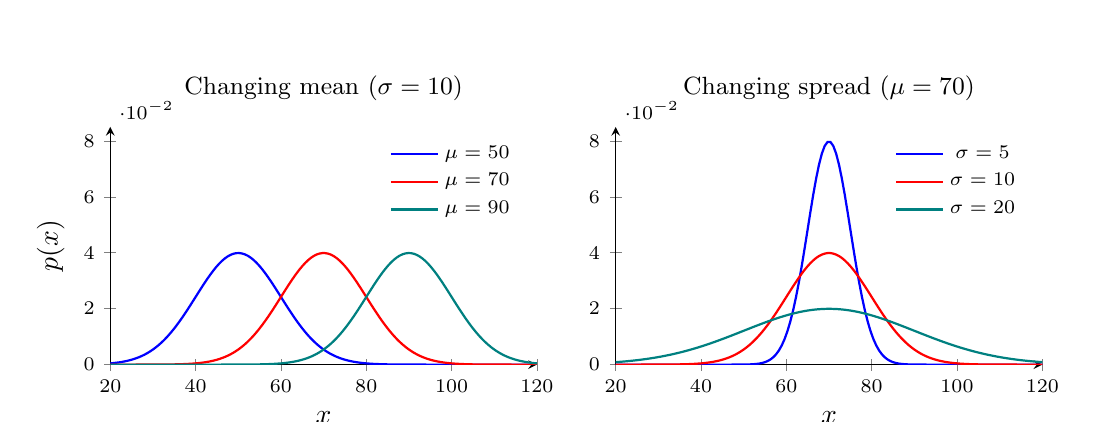
\begin{tikzpicture}
\begin{axis}[name=a,width=7cm,height=4.6cm,xmin=20,xmax=120,ymin=0,ymax=0.085,
  title={\small Changing mean ($\sigma=10$)},xlabel={$x$},ylabel={$p(x)$},axis lines=left,
  samples=150,domain=20:120,legend style={font=\scriptsize,draw=none},legend pos=north east,
  yticklabel style={/pgf/number format/fixed,font=\scriptsize},xticklabel style={font=\scriptsize}]
\addplot[blue,thick]{exp(-(x-50)^2/200)/sqrt(200*pi)};
\addplot[red,thick]{exp(-(x-70)^2/200)/sqrt(200*pi)};
\addplot[teal,thick]{exp(-(x-90)^2/200)/sqrt(200*pi)};
\legend{{$\mu=50$},{$\mu=70$},{$\mu=90$}}
\end{axis}
\begin{axis}[at={(a.east)},anchor=west,xshift=1.0cm,width=7cm,height=4.6cm,xmin=20,xmax=120,ymin=0,ymax=0.085,
  title={\small Changing spread ($\mu=70$)},xlabel={$x$},axis lines=left,
  samples=150,domain=20:120,legend style={font=\scriptsize,draw=none},legend pos=north east,
  yticklabel style={/pgf/number format/fixed,font=\scriptsize},xticklabel style={font=\scriptsize}]
\addplot[blue,thick]{exp(-(x-70)^2/50)/sqrt(50*pi)};
\addplot[red,thick]{exp(-(x-70)^2/200)/sqrt(200*pi)};
\addplot[teal,thick]{exp(-(x-70)^2/800)/sqrt(800*pi)};
\legend{{$\sigma=5$},{$\sigma=10$},{$\sigma=20$}}
\end{axis}
\end{tikzpicture}
\end{center}
Changing $\mu$ slides the curve left or right. Changing $\sigma$ makes it wider \emph{and} lower (the area must stay $1$): the peak height is $1/\sqrt{2\pi\sigma^2}$, i.e.\ $0.0798$, $0.0399$ and $0.0199$ for $\sigma=5,10,20$.

\begin{example}[Example 1.1: Examination marks and the 68--95 rule]
Marks follow $x\sim\N(70,10^2)$: mean $70$, standard deviation $10$, variance $100$.

\begin{center}
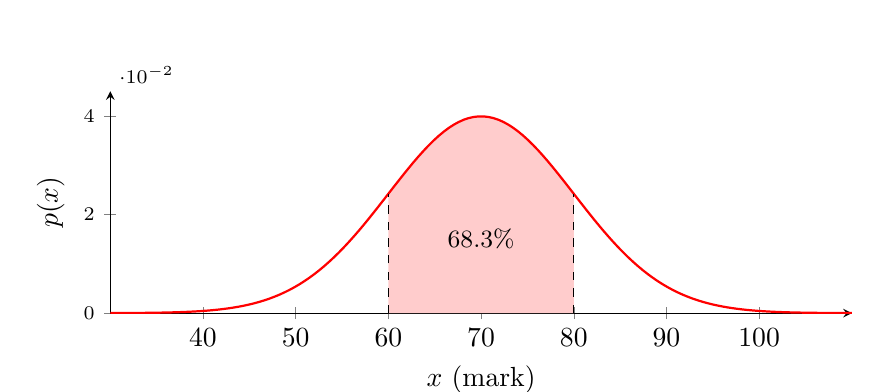
\begin{tikzpicture}
\begin{axis}[width=11cm,height=4.4cm,xmin=30,xmax=110,ymin=0,ymax=0.045,axis lines=left,
  xlabel={$x$ (mark)},ylabel={$p(x)$},samples=150,domain=30:110,xtick={40,50,60,70,80,90,100},
  yticklabel style={/pgf/number format/fixed,font=\scriptsize}]
\addplot[name path=f,red,thick]{exp(-(x-70)^2/200)/sqrt(200*pi)};
\path[name path=axis] (axis cs:30,0) -- (axis cs:110,0);
\addplot[fill=red!20] fill between[of=f and axis,soft clip={domain=60:80}];
\node at (axis cs:70,0.015) {\small 68.3\%};
\draw[dashed] (axis cs:60,0)--(axis cs:60,0.0242) (axis cs:80,0)--(axis cs:80,0.0242);
\end{axis}
\end{tikzpicture}
\end{center}

To find a probability, convert to a \textbf{z-score} $z=(x-\mu)/\sigma$, which counts standard deviations from the mean.
\begin{itemize}[nosep]
\item $60\le x\le80 \iff -1\le z\le1$: probability $\approx68.3\%$.
\item $50\le x\le90 \iff -2\le z\le2$: probability $\approx95.4\%$.
\item $40\le x\le100\iff -3\le z\le3$: probability $\approx99.7\%$.
\end{itemize}
\textbf{Extra question:} what fraction of students score above $85$? $z=(85-70)/10=1.5$, and $P(Z>1.5)=0.0668$, so about $6.7\%$.

\textbf{Density at a point:} $\N(74\mid70,100)=\dfrac{1}{\sqrt{200\pi}}e^{-16/200}=0.039894\times e^{-0.08}=0.039894\times0.92312=0.036827$.
\end{example}

\begin{caution}[Density is not probability]
$p(74)=0.0368$ is a \emph{density}, not ``the probability of scoring exactly 74'' (that is $0$ for a continuous variable). Probabilities are \emph{areas} under the curve. Densities can even exceed $1$ when $\sigma$ is small (e.g.\ $\sigma=0.1$ gives a peak of $3.99$). This fact matters later in Section~\ref{sec:degenerate}.
\end{caution}

%======================================================================
\section{From One Gaussian to a Mixture}
%======================================================================

\subsection{The mixture model}

One Gaussian models \emph{one} cluster. Real data often contain several, for example marks from three groups of students. A Gaussian Mixture Model (GMM) combines $K$ Gaussians into one distribution:
\[
\boxed{\;p(x)=\sum_{k=1}^K\pi_k\,\N(x\mid\mu_k,\sigma_k^2)\;}
\]
\begin{itemize}[nosep]
\item $K$: number of components;
\item $\pi_k$: \textbf{mixing probability} (weight) of component $k$;
\item $\mu_k$, $\sigma_k^2$: mean and variance of component $k$.
\end{itemize}

\textbf{Mixing probabilities} say how much each component contributes. They must form a probability distribution:
\[
\pi_k\ge0\ \text{for all }k,\qquad\sum_{k=1}^K\pi_k=1.
\]
\emph{Why must they sum to 1?} Each $\N(\cdot)$ integrates to $1$, so $\int p(x)\,dx=\sum_k\pi_k\cdot1=\sum_k\pi_k$. For $p(x)$ to be a valid density this must equal $1$.

\subsection{The running three-group example}

\begin{center}
\begin{tabular}{@{}clccc@{}}
\toprule
Component & Student group & Mean $\mu_k$ & Std.\ dev.\ $\sigma_k$ & Mixing prob.\ $\pi_k$\\
\midrule
1 & Lower-performing & 50 & 5 & 0.30\\
2 & Average-performing & 70 & 10 & 0.50\\
3 & Higher-performing & 90 & 5 & 0.20\\
\midrule
& Total & & & 1.00\\
\bottomrule
\end{tabular}
\end{center}
For 1{,}000 students we would expect about $300$, $500$ and $200$ in the three groups. The GMM does \emph{not} need to know each student's group; it \emph{estimates} the components from the data.

\begin{center}
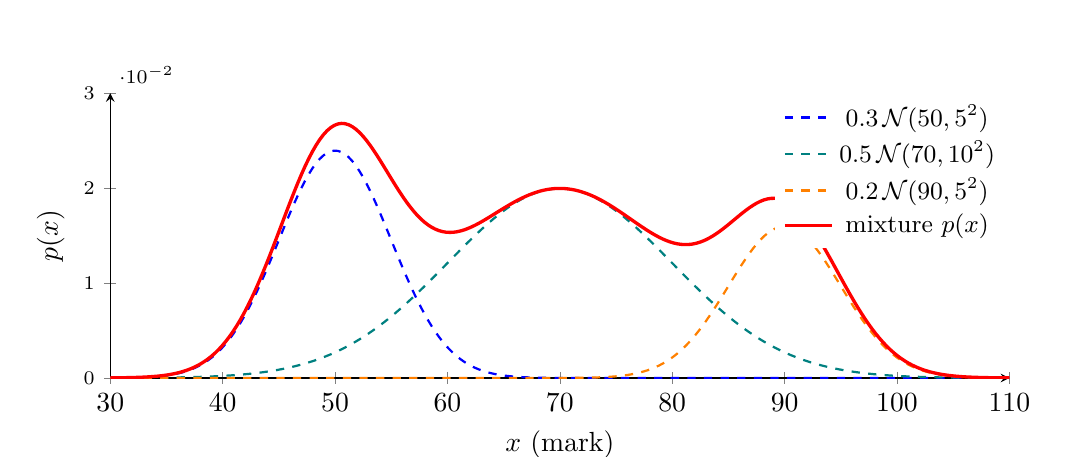
\begin{tikzpicture}
\begin{axis}[width=13cm,height=5.2cm,xmin=30,xmax=110,ymin=0,ymax=0.03,axis lines=left,
  xlabel={$x$ (mark)},ylabel={$p(x)$},samples=250,domain=30:110,
  legend style={font=\small,draw=none,at={(1,1)},anchor=north east},
  yticklabel style={/pgf/number format/fixed,font=\scriptsize}]
\addplot[blue,dashed,thick]{0.3*exp(-(x-50)^2/50)/sqrt(50*pi)};
\addplot[teal,dashed,thick]{0.5*exp(-(x-70)^2/200)/sqrt(200*pi)};
\addplot[orange,dashed,thick]{0.2*exp(-(x-90)^2/50)/sqrt(50*pi)};
\addplot[red,very thick]{0.3*exp(-(x-50)^2/50)/sqrt(50*pi)+0.5*exp(-(x-70)^2/200)/sqrt(200*pi)+0.2*exp(-(x-90)^2/50)/sqrt(50*pi)};
\legend{{$0.3\,\N(50,5^2)$},{$0.5\,\N(70,10^2)$},{$0.2\,\N(90,5^2)$},{mixture $p(x)$}}
\end{axis}
\end{tikzpicture}
\end{center}
Dashed curves are the \emph{weighted} components $\pi_k\N(x\mid\mu_k,\sigma_k^2)$; the red curve is their sum. Note that component 2 has the largest weight but, being wide, a lower and broader bump.

\begin{example}[Example 2.1: Evaluating the mixture density at $x=60$]
Compute each Gaussian, weight it, and add.
\begin{align*}
\N(60\mid50,25)&=\tfrac{1}{\sqrt{50\pi}}e^{-100/50}=0.079788\times e^{-2}=0.010798,\\
\N(60\mid70,100)&=\tfrac{1}{\sqrt{200\pi}}e^{-100/200}=0.039894\times e^{-0.5}=0.024197,\\
\N(60\mid90,25)&=0.079788\times e^{-900/50}=0.079788\times e^{-18}\approx1.2\times10^{-9}.
\end{align*}
\[
p(60)=0.3(0.010798)+0.5(0.024197)+0.2(1.2\times10^{-9})\approx0.003239+0.012099=\mathbf{0.015338}.
\]
Notice $60$ is exactly $2\sigma$ from $\mu_1=50$ but only $1\sigma$ from $\mu_2=70$; distance must always be judged relative to each component's own $\sigma$.
\end{example}

%======================================================================
\section{Generative Interpretation}
%======================================================================

A GMM is a \emph{recipe} for generating data. This is why it is called a \textbf{generative} model.

\begin{center}
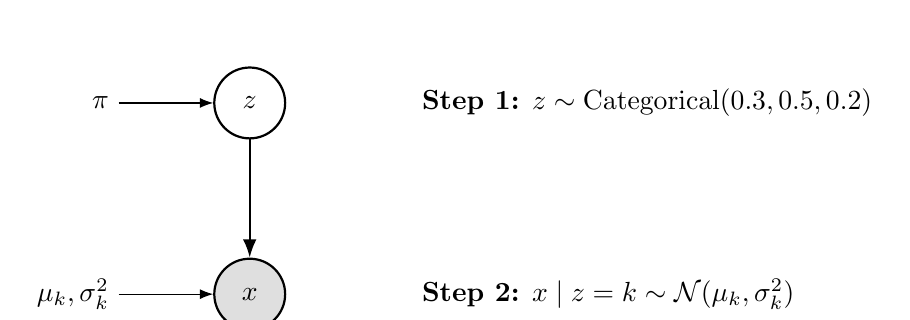
\begin{tikzpicture}[node distance=1.5cm,
  latent/.style={circle,draw,thick,minimum size=9mm},
  obs/.style={circle,draw,thick,fill=gray!25,minimum size=9mm}]
\node[latent] (z) {$z$};
\node[obs,below=of z] (x) {$x$};
\node[left=1.2cm of z] (pi) {$\pi$};
\node[left=1.2cm of x] (mu) {$\mu_k,\sigma_k^2$};
\draw[-{Latex},thick] (z)--(x);
\draw[-{Latex}] (pi)--(z);
\draw[-{Latex}] (mu)--(x);
\node[right=1.6cm of z,align=left] {\textbf{Step 1:} $z\sim\mathrm{Categorical}(0.3,0.5,0.2)$};
\node[right=1.6cm of x,align=left] {\textbf{Step 2:} $x\mid z=k\sim\N(\mu_k,\sigma_k^2)$};
\end{tikzpicture}
\end{center}

\textbf{Step 1 -- select a component.} Draw the hidden (latent) label $z$ with probabilities $\pi$.\\
\textbf{Step 2 -- generate an observation.} Draw $x$ from the chosen Gaussian:
\[
x\mid z=1\sim\N(50,25),\qquad x\mid z=2\sim\N(70,100),\qquad x\mid z=3\sim\N(90,25).
\]
(The second argument is the \emph{variance}: $5^2=25$ and $10^2=100$.)

\begin{example}[Example 3.1: Generating one mark by hand]
\textbf{Step 1.} Draw $u\sim\mathrm{Uniform}(0,1)$, say $u=0.47$. Cumulative weights are $0.30,\;0.80,\;1.00$. Since $0.30<0.47\le0.80$, choose $z=2$.

\textbf{Step 2.} Draw a standard normal $\epsilon$, say $\epsilon=0.4$, and set $x=\mu_2+\sigma_2\epsilon=70+10(0.4)=74$.

This reproduces the handout's example: component 2 was selected and the mark $x=74$ was generated. Repeating this $1{,}000$ times gives a histogram shaped like the red mixture curve.
\end{example}

\textbf{Step 3 -- joint and marginal.} The joint probability of a mark and its component is prior $\times$ likelihood:
\[
p(x,z=k)=p(z=k)\,p(x\mid z=k)=\pi_k\,\N(x\mid\mu_k,\sigma_k^2).
\]
We never observe $z$, so we \emph{marginalise} (sum it out) by the sum rule of probability:
\[
p(x)=\sum_{k=1}^Kp(x,z=k)=\sum_{k=1}^K\pi_k\,\N(x\mid\mu_k,\sigma_k^2),
\]
which is exactly the GMM formula. So ``a GMM'' and ``a two-step generative process with a hidden label'' are the same model.

\textbf{Step 4 -- generation vs.\ inference.}
\begin{center}
\begin{tabular}{@{}ll@{}}
\toprule
Generative process & Inference process\\
\midrule
Select component $z$ & Observe mark $x$\\
Generate mark $x$ & Estimate component $z$\\
Uses mixing probability $\pi_k$ & Uses posterior probability $p(z=k\mid x)$\\
Forward direction ($z\to x$) & Reverse direction ($x\to z$)\\
\bottomrule
\end{tabular}
\end{center}
Generation runs forward from cause to data. Inference runs backward: given a mark, which group was it \emph{probably} from? Bayes' theorem reverses the arrow.

%======================================================================
\section{Posterior Probability and Responsibilities}
%======================================================================

By Bayes' theorem,
\[
p(z=k\mid x)=\frac{p(x\mid z=k)\,p(z=k)}{p(x)},
\]
with, in a GMM,
\begin{itemize}[nosep]
\item $p(z=k)=\pi_k$: \textbf{prior} (mixing probability), before seeing the mark;
\item $p(x\mid z=k)=\N(x\mid\mu_k,\sigma_k^2)$: \textbf{likelihood}, how well group $k$ explains the mark;
\item $p(x)=\sum_j\pi_j\N(x\mid\mu_j,\sigma_j^2)$: \textbf{evidence} (marginal likelihood);
\item $p(z=k\mid x)$: \textbf{posterior}, also called the \textbf{responsibility} $r_k(x)$.
\end{itemize}
\[
\boxed{\;r_k(x)=p(z=k\mid x)=\frac{\pi_k\,\N(x\mid\mu_k,\sigma_k^2)}{\sum_{j=1}^K\pi_j\,\N(x\mid\mu_j,\sigma_j^2)}\;}
\]
Recipe: (1) compute the \emph{weighted likelihood} $w_k=\pi_k\N(x\mid\mu_k,\sigma_k^2)$ for every $k$; (2) divide each by their sum. Responsibilities are between $0$ and $1$ and sum to $1$ over $k$.

\begin{example}[Example 4.1: Which group does a mark of 74 belong to? (handout example)]
\textbf{Step 1 -- weighted likelihoods.}
\begin{align*}
w_1&=0.3\times\N(74\mid50,25)=0.3\times0.079788\,e^{-24^2/50}=0.3\times7.92\times10^{-7}=2.38\times10^{-7},\\
w_2&=0.5\times\N(74\mid70,100)=0.5\times0.039894\,e^{-0.08}=0.5\times0.036827=0.018414,\\
w_3&=0.2\times\N(74\mid90,25)=0.2\times0.079788\,e^{-16^2/50}=0.2\times4.77\times10^{-4}=9.54\times10^{-5}.
\end{align*}
\textbf{Step 2 -- normalise.} Sum $=0.000000238+0.018414+0.000095=0.018509$ (this is $p(74)$).
\begin{center}
\begin{tabular}{@{}ccc@{}}
\toprule
Component & $w_k$ & $r_k(74)=w_k/0.018509$\\
\midrule
1 & 0.000000238 & 0.00001\\
2 & 0.018414 & 0.99483\\
3 & 0.000095 & 0.00515\\
\midrule
Total & 0.018509 & 1.00000\\
\bottomrule
\end{tabular}
\end{center}
\textbf{Conclusion:} a mark of 74 almost certainly came from the average group ($99.5\%$).
\end{example}

\begin{example}[Example 4.2: Borderline marks (extra)]
The same recipe for other marks:
\begin{center}
\begin{tabular}{@{}cccccl@{}}
\toprule
Mark $x$ & $p(x)$ & $r_1(x)$ & $r_2(x)$ & $r_3(x)$ & Comment\\
\midrule
60 & 0.015338 & 0.2112 & 0.7888 & 0.0000 & ambiguous between groups 1 and 2\\
62 & 0.015828 & 0.0849 & 0.9151 & 0.0000 & 2 marks higher, group 1 fades fast\\
80 & 0.014258 & 0.0000 & 0.8485 & 0.1515 & mostly group 2\\
85 & 0.016155 & 0.0000 & 0.4009 & 0.5991 & group 3 just wins\\
\bottomrule
\end{tabular}
\end{center}
\textbf{Worked line for $x=85$:}
$w_2=0.5\times0.039894\,e^{-225/200}=0.5\times0.012952=0.006476$ and
$w_3=0.2\times0.079788\,e^{-25/50}=0.2\times0.048394=0.009679$, so
$r_3=0.009679/(0.006476+0.009679)=0.599$.

\textbf{Lesson:} $85$ is $5$ marks from $\mu_3$ ($1\sigma_3$) and $15$ from $\mu_2$ ($1.5\sigma_2$). Group 3's narrow, tall Gaussian gives a likelihood almost $4\times$ larger, which beats group 2's larger prior ($0.5$ vs.\ $0.2$) only narrowly. Prior and likelihood \emph{both} matter.
\end{example}

%======================================================================
\section{The Expectation--Maximization (EM) Algorithm}
%======================================================================

\subsection{Problem formulation}

So far the parameters were \emph{given}. In practice we only have marks $X=\{x_1,\dots,x_N\}$ and do not know $\pi_k$, $\mu_k$, $\sigma_k^2$, \emph{or} which component produced each mark. The unknown parameters are
\[
\theta=\{\pi_k,\mu_k,\sigma_k^2\}_{k=1}^K,
\]
and we want the \textbf{maximum likelihood estimate} (MLE)
$\theta_{\text{MLE}}=\arg\max_\theta p(X\mid\theta)$.

\subsection{Likelihood of the observed data}

If marks are independent, their joint probability is a product, and the log turns it into a sum:
\[
p(X\mid\theta)=\prod_{n=1}^N\Big[\sum_{k=1}^K\pi_k\N(x_n\mid\mu_k,\sigma_k^2)\Big],
\qquad
\boxed{\;\LL(\theta)=\sum_{n=1}^N\log\Big[\sum_{k=1}^K\pi_k\N(x_n\mid\mu_k,\sigma_k^2)\Big].\;}
\]
The data $X$ are fixed; $\LL$ is a function of $\theta$ only. We use the log because a product of many small numbers underflows to $0$ on a computer, and sums are easier to differentiate.

\subsection{Why direct estimation is difficult}

\begin{itemize}[nosep]
\item The log is applied to a \emph{sum}, and $\log(a+b)\ne\log a+\log b$, so it does not simplify.
\item The parameters of different components are \emph{coupled} inside that sum.
\item Setting $\partial\LL/\partial\mu_k=0$ gives an equation in which $\mu_k$ appears on both sides (through the responsibilities): there is no closed-form maximiser.
\end{itemize}
Contrast this with one Gaussian ($K=1$), where $\log\N$ is a simple quadratic and the answer is just the sample mean and variance.

\subsection{The central idea of EM}

\begin{keyidea}[The chicken-and-egg problem]
If we knew the \emph{groups}, estimating the parameters would be easy (average each group). If we knew the \emph{parameters}, estimating the groups would be easy (Bayes' rule). EM breaks the deadlock by alternating:
\begin{itemize}[nosep]
\item \textbf{E-step (Expectation):} with the current $\theta$, compute responsibilities $r_{nk}=p(z_n=k\mid x_n,\theta)$.
\item \textbf{M-step (Maximization):} with those responsibilities, re-estimate $\pi_k,\mu_k,\sigma_k^2$ as \emph{weighted} averages.
\end{itemize}
Repeat until convergence.
\end{keyidea}

\begin{center}
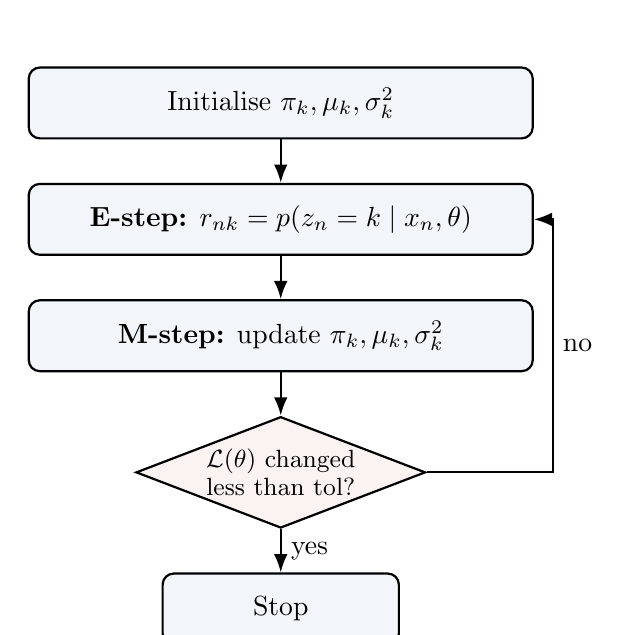
\begin{tikzpicture}[node distance=0.55cm,
  box/.style={draw,thick,rounded corners,align=center,minimum width=6.4cm,minimum height=9mm,fill=idea!6},
  dec/.style={draw,thick,diamond,aspect=2.6,align=center,fill=warn!6,inner sep=1pt}]
\node[box] (init) {Initialise $\pi_k,\mu_k,\sigma_k^2$};
\node[box,below=of init] (e) {\textbf{E-step:} $r_{nk}=p(z_n=k\mid x_n,\theta)$};
\node[box,below=of e] (m) {\textbf{M-step:} update $\pi_k,\mu_k,\sigma_k^2$};
\node[dec,below=of m] (c) {\small$\LL(\theta)$ changed\\[-2pt]\small less than tol?};
\node[box,below=of c,minimum width=3cm] (stop) {Stop};
\draw[-{Latex},thick] (init)--(e);
\draw[-{Latex},thick] (e)--(m);
\draw[-{Latex},thick] (m)--(c);
\draw[-{Latex},thick] (c)--node[right]{yes}(stop);
\draw[-{Latex},thick] (c.east)--++(1.6,0)|-node[pos=0.25,right]{no}(e.east);
\end{tikzpicture}
\end{center}

\subsection{M-step: updating the GMM parameters}

\textbf{Effective number of observations.}
\[
N_k=\sum_{n=1}^N r_{nk}.
\]
$N_k$ is a ``soft count'': a point with $r_{nk}=0.8$ counts as $0.8$ of an observation for component $k$. It need not be an integer, and since every row of responsibilities sums to $1$,
\[
\sum_kN_k=\sum_n\sum_kr_{nk}=\sum_n1=N.
\]

\textbf{Update the mixing probabilities, means and variances.}
\[
\pi_k^{\text{new}}=\frac{N_k}{N},\qquad
\mu_k^{\text{new}}=\frac{1}{N_k}\sum_{n=1}^N r_{nk}\,x_n,\qquad
(\sigma_k^2)^{\text{new}}=\frac{1}{N_k}\sum_{n=1}^N r_{nk}\,\big(x_n-\mu_k^{\text{new}}\big)^2.
\]
\begin{itemize}[nosep]
\item $\pi_k$: fraction of the (soft) data owned by component $k$.
\item $\mu_k$: responsibility-weighted average of the marks.
\item $\sigma_k^2$: responsibility-weighted spread around the \emph{new} mean.
\end{itemize}
If all $r_{nk}$ were $0$ or $1$, these reduce to the ordinary count, mean and variance of each group.

\textbf{Where they come from (sketch).} Holding $r_{nk}$ fixed, the M-step maximises
\[
Q(\theta)=\sum_n\sum_kr_{nk}\Big[\log\pi_k-\tfrac12\log(2\pi\sigma_k^2)-\frac{(x_n-\mu_k)^2}{2\sigma_k^2}\Big].
\]
\begin{itemize}[leftmargin=*]
\item $\dfrac{\partial Q}{\partial\mu_k}=\sum_nr_{nk}\dfrac{x_n-\mu_k}{\sigma_k^2}=0\;\Rightarrow\;\mu_k=\dfrac{\sum_nr_{nk}x_n}{N_k}$.
\item $\dfrac{\partial Q}{\partial\sigma_k^2}=\sum_nr_{nk}\Big[-\dfrac{1}{2\sigma_k^2}+\dfrac{(x_n-\mu_k)^2}{2\sigma_k^4}\Big]=0\;\Rightarrow\;\sigma_k^2=\dfrac{\sum_nr_{nk}(x_n-\mu_k)^2}{N_k}$.
\item For $\pi_k$, maximise $\sum_kN_k\log\pi_k$ subject to $\sum_k\pi_k=1$ (Lagrange multiplier $\lambda$): $N_k/\pi_k=\lambda$, and summing gives $\lambda=N$, so $\pi_k=N_k/N$.
\end{itemize}

\subsection{Summary of the complete algorithm}

\begin{center}
\begin{tabular}{@{}ll@{}}
\toprule
Quantity & Update equation\\
\midrule
Responsibility (E) & $r_{nk}=\pi_k\N(x_n\mid\mu_k,\sigma_k^2)\big/\sum_j\pi_j\N(x_n\mid\mu_j,\sigma_j^2)$\\
Effective count & $N_k=\sum_nr_{nk}$\\
Mixing probability & $\pi_k=N_k/N$\\
Mean & $\mu_k=\frac1{N_k}\sum_nr_{nk}x_n$\\
Variance & $\sigma_k^2=\frac1{N_k}\sum_nr_{nk}(x_n-\mu_k)^2$\\
\bottomrule
\end{tabular}
\end{center}
\begin{enumerate}[nosep]
\item Initialise $\pi_k,\mu_k,\sigma_k^2$.
\item E-step: compute $r_{nk}$ for every observation and component.
\item M-step: update the mixing probabilities, means and variances.
\item Compute the log-likelihood $\LL(\theta)$.
\item Repeat 2--4 until $\LL$ (or the parameters) stop changing appreciably.
\end{enumerate}
\begin{keyidea}[Important]
Each EM iteration \textbf{never decreases} $\LL(\theta)$, but EM may converge to a \textbf{local} maximum, so the result can depend on the initialisation. (The proof uses the ELBO; see the Lecture 2 notes, Section 3.5.)
\end{keyidea}

%======================================================================
\section{EM by Hand: A Full Numerical Example}
%======================================================================

\subsection{Problem definition}

Five marks, two components:
\[
X=\{50,\,55,\,70,\,75,\,80\},\qquad N=5,\qquad K=2.
\]
\begin{center}
\begin{tabular}{@{}lcc@{}}
\toprule
Parameter & Component 1 & Component 2\\
\midrule
Mixing probability $\pi_k$ & 0.5 & 0.5\\
Mean $\mu_k$ & 50 & 80\\
Variance $\sigma_k^2$ & 100 & 100\\
\bottomrule
\end{tabular}
\end{center}
With $\sigma^2=100$:
$\N(x\mid\mu,100)=\dfrac{1}{\sqrt{200\pi}}\exp\!\Big[-\dfrac{(x-\mu)^2}{200}\Big]$, and $\dfrac{1}{\sqrt{200\pi}}=0.039894$.

\subsection{Log-likelihood at the start (filled in)}

The handout states $\LL(\theta^{(0)})=-20.003$. Here is how to get it. For each mark, $p(x_n)=0.5\N(x_n\mid50,100)+0.5\N(x_n\mid80,100)$:
\begin{center}
\begin{tabular}{@{}ccccc@{}}
\toprule
$x_n$ & $\N(x_n\mid50,100)$ & $\N(x_n\mid80,100)$ & $p(x_n)$ & $\log p(x_n)$\\
\midrule
50 & 0.039894 & 0.000443 & 0.020169 & $-3.9036$\\
55 & 0.035207 & 0.001753 & 0.018480 & $-3.9911$\\
70 & 0.005399 & 0.024197 & 0.014798 & $-4.2133$\\
75 & 0.001753 & 0.035207 & 0.018480 & $-3.9911$\\
80 & 0.000443 & 0.039894 & 0.020169 & $-3.9036$\\
\midrule
& & & Sum $=\LL(\theta^{(0)})$ & $\mathbf{-20.0027}$\\
\bottomrule
\end{tabular}
\end{center}
Exponents used: $(55-50)^2/200=0.125$, $(55-80)^2/200=3.125$, $(70-50)^2/200=2$, $(70-80)^2/200=0.5$, $(50-80)^2/200=4.5$.

\subsection{E-step}

For two components with equal weights,
\[
r_{n1}=\frac{0.5\,\N(x_n\mid50,100)}{0.5\,\N(x_n\mid50,100)+0.5\,\N(x_n\mid80,100)},\qquad r_{n2}=1-r_{n1}.
\]

\begin{example}[Example 6.1: Responsibilities for three of the marks]
\textbf{$x=50$ (handout):} $w_1=0.5(0.039894)=0.019947$, $w_2=0.5(0.000443)=0.000222$,
\[
r_{11}=\frac{0.019947}{0.019947+0.000222}=0.98901,\qquad r_{12}=0.01099.
\]
\textbf{$x=55$:} $w_1=0.5(0.035207)=0.017604$, $w_2=0.5(0.001753)=0.000877$,
\[
r_{21}=\frac{0.017604}{0.017604+0.000877}=0.95257,\qquad r_{22}=0.04743.
\]
\textbf{$x=70$:} $w_1=0.5(0.005399)=0.002700$, $w_2=0.5(0.024197)=0.012099$,
\[
r_{31}=\frac{0.002700}{0.002700+0.012099}=0.18243,\qquad r_{32}=0.81757.
\]
\textbf{Shortcut:} with equal weights and variances, $\pi$ and the constant cancel, so
$r_{n1}=1/\big(1+e^{-[(x_n-80)^2-(x_n-50)^2]/200}\big)$. For $x=70$: exponent $=-(100-400)/200=1.5$, so $r_{31}=1/(1+e^{1.5})=1/(1+4.4817)=0.18243$.

By symmetry ($75$ mirrors $55$ and $80$ mirrors $50$ about $65$) the remaining rows are swapped.
\end{example}

\begin{center}
\begin{tabular}{@{}ccc@{}}
\toprule
$x_n$ & $r_{n1}$ & $r_{n2}$\\
\midrule
50 & 0.98901 & 0.01099\\
55 & 0.95257 & 0.04743\\
70 & 0.18243 & 0.81757\\
75 & 0.04743 & 0.95257\\
80 & 0.01099 & 0.98901\\
\midrule
Sum & 2.18243 & 2.81757\\
\bottomrule
\end{tabular}
\end{center}
Each row sums to one. These are \textbf{soft assignments}: each mark contributes to \emph{both} components in proportion to its responsibilities.

\subsection{M-step}

\textbf{Step 1 -- effective counts.}
\[
N_1=0.98901+0.95257+0.18243+0.04743+0.01099=2.18243,\qquad N_2=2.81757,\qquad N_1+N_2=5.
\]
Component 2 owns more data because the mark $70$ (between the initial means) leans towards $80$.

\textbf{Step 2 -- mixing probabilities.}
\[
\pi_1^{(1)}=\frac{2.18243}{5}=0.43649,\qquad\pi_2^{(1)}=\frac{2.81757}{5}=0.56351.
\]

\textbf{Step 3 -- means.}
\[
\mu_1^{(1)}=\frac{0.98901(50)+0.95257(55)+0.18243(70)+0.04743(75)+0.01099(80)}{2.18243}=\frac{119.048}{2.18243}=54.55,
\]
\[
\mu_2^{(1)}=\frac{0.01099(50)+0.04743(55)+0.81757(70)+0.95257(75)+0.98901(80)}{2.81757}=\frac{210.952}{2.81757}=74.87.
\]

\textbf{Step 4 -- variances (individual terms filled in).} Use the \emph{new} means.
\begin{center}
\begin{tabular}{@{}ccc@{}}
\toprule
$x_n$ & $r_{n1}(x_n-54.548)^2$ & $r_{n2}(x_n-74.870)^2$\\
\midrule
50 & $0.98901\times20.69=20.461$ & $0.01099\times618.52=6.796$\\
55 & $0.95257\times0.204=0.194$ & $0.04743\times394.82=18.725$\\
70 & $0.18243\times238.75=43.554$ & $0.81757\times23.72=19.391$\\
75 & $0.04743\times418.27=19.837$ & $0.95257\times0.017=0.016$\\
80 & $0.01099\times647.78=7.117$ & $0.98901\times26.32=26.027$\\
\midrule
Sum & $91.163$ & $70.954$\\
\bottomrule
\end{tabular}
\end{center}
\[
(\sigma_1^2)^{(1)}=\frac{91.163}{2.18243}=41.77,\qquad(\sigma_2^2)^{(1)}=\frac{70.954}{2.81757}=25.18.
\]
Note that the mark $70$ contributes the \emph{largest} term to component 1's variance even though $r_{31}$ is only $0.18$, because it is far from $\mu_1$.

\subsection{Parameters after one iteration}

\begin{center}
\begin{tabular}{@{}lcc@{}}
\toprule
Parameter & Initial & After iteration 1\\
\midrule
$\pi_1$ & 0.50000 & 0.43649\\
$\pi_2$ & 0.50000 & 0.56351\\
$\mu_1$ & 50 & 54.55\\
$\mu_2$ & 80 & 74.87\\
$\sigma_1^2$ & 100 & 41.77\\
$\sigma_2^2$ & 100 & 25.18\\
Log-likelihood $\LL(\theta)$ & $-20.003$ & $-17.730$\\
\bottomrule
\end{tabular}
\end{center}
The log-likelihood rose, as EM guarantees. The means moved towards the natural clusters $\{50,55\}$ and $\{70,75,80\}$, and the variances shrank to fit them more tightly.

\subsection{What happens next? (iterations 2 and beyond, filled in)}

\begin{example}[Example 6.2: Second iteration]
\textbf{E-step} with $\theta^{(1)}$: the narrower Gaussians make the responsibilities sharper.
\begin{center}
\begin{tabular}{@{}cccccc@{}}
\toprule
$x_n$ & 50 & 55 & 70 & 75 & 80\\
\midrule
$r_{n1}$ & 0.99999 & 0.99934 & 0.05238 & 0.00401 & 0.00043\\
$r_{n2}$ & 0.00001 & 0.00066 & 0.94762 & 0.99599 & 0.99957\\
\bottomrule
\end{tabular}
\end{center}
The mark $70$ has moved decisively to component 2 ($0.18\to0.05$ for component 1).

\textbf{M-step:}
$N=(2.0562,\,2.9438)$, $\pi=(0.41123,\,0.58877)$,
$\mu_1=108.966/2.0562=52.99$, $\mu_2=221.034/2.9438=75.08$,
$\sigma_1^2=30.394/2.0562=14.78$, $\sigma_2^2=48.928/2.9438=16.62$.
Log-likelihood: $-16.815$.
\end{example}

\begin{center}
\begin{tabular}{@{}lccccccc@{}}
\toprule
Iteration & $\pi_1$ & $\pi_2$ & $\mu_1$ & $\mu_2$ & $\sigma_1^2$ & $\sigma_2^2$ & $\LL(\theta)$\\
\midrule
0 (initial) & 0.500 & 0.500 & 50.00 & 80.00 & 100.00 & 100.00 & $-20.003$\\
1 & 0.436 & 0.564 & 54.55 & 74.87 & 41.77 & 25.18 & $-17.730$\\
2 & 0.411 & 0.589 & 52.99 & 75.08 & 14.78 & 16.62 & $-16.815$\\
3 onwards (converged) & 0.400 & 0.600 & 52.50 & 75.00 & 6.25 & 16.67 & $-16.512$\\
\bottomrule
\end{tabular}
\end{center}

\begin{center}
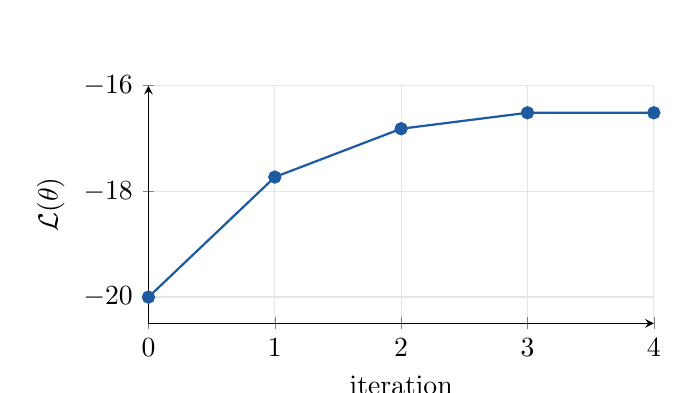
\begin{tikzpicture}
\begin{axis}[width=8cm,height=4.6cm,xlabel={iteration},ylabel={$\LL(\theta)$},axis lines=left,
  xtick={0,1,2,3,4},ymin=-20.5,ymax=-16,mark size=2pt,grid=major,grid style={gray!20}]
\addplot[idea,thick,mark=*] coordinates {(0,-20.0027) (1,-17.7297) (2,-16.8145) (3,-16.5124) (4,-16.5124)};
\end{axis}
\end{tikzpicture}
\end{center}

\textbf{Interpreting the converged answer.} The final model is exactly the ``obvious'' grouping:
\begin{itemize}[nosep]
\item Component 1 $=\{50,55\}$: $\pi_1=2/5=0.4$, mean $52.5$, variance $\frac{(2.5)^2+(2.5)^2}{2}=6.25$.
\item Component 2 $=\{70,75,80\}$: $\pi_2=3/5=0.6$, mean $75$, variance $\frac{25+0+25}{3}=16.67$.
\end{itemize}
Because the two clusters are well separated, the responsibilities become (almost) $0$ or $1$, and EM's soft answer coincides with the hard one. The log-likelihood climbs quickly at first and then flattens: most of the improvement comes in the first two iterations.

\subsection{GMM-EM vs.\ \texorpdfstring{$k$}{k}-means on the same data}

\begin{example}[Example 6.3: $k$-means with the same starting centres]
$k$-means uses \textbf{hard} assignments: each point goes to its nearest centre.

\textbf{Iteration 1.} Centres $c_1=50$, $c_2=80$.
\begin{center}
\begin{tabular}{@{}cccc@{}}
\toprule
$x_n$ & $|x_n-50|$ & $|x_n-80|$ & assigned to\\
\midrule
50 & 0 & 30 & 1\\
55 & 5 & 25 & 1\\
70 & 20 & 10 & 2\\
75 & 25 & 5 & 2\\
80 & 30 & 0 & 2\\
\bottomrule
\end{tabular}
\end{center}
New centres: $c_1=(50+55)/2=52.5$, $c_2=(70+75+80)/3=75$.

\textbf{Iteration 2.} The assignments do not change, so $k$-means stops at $(52.5,\,75)$.
\end{example}

\begin{center}
\begin{tabular}{@{}p{3.6cm}p{5.2cm}p{5.6cm}@{}}
\toprule
& $k$-means & GMM with EM\\
\midrule
Assignment & Hard (0 or 1) & Soft ($0\le r_{nk}\le1$)\\
Learns & Centres only & Means, variances, weights\\
Cluster shape & Equal-sized spheres (implicitly) & Each component has its own spread\\
Objective & Within-cluster squared distance & Log-likelihood\\
Output for $x=70$ at iteration 1 & ``Cluster 2'' & ``$18\%$ cluster 1, $82\%$ cluster 2''\\
Relationship & Limit of EM with $\sigma_k^2=\epsilon\to0$ & General case\\
\bottomrule
\end{tabular}
\end{center}
On this well-separated data both reach the same means. $k$-means is cheaper and is a good way to \emph{initialise} EM.

\subsection{Key learning points}
\begin{enumerate}[nosep]
\item The \textbf{E-step} estimates the probability that each observation belongs to each component.
\item The \textbf{M-step} updates the mixing probabilities, means and variances using those probabilities as weights.
\item $N_k$ is the effective number of observations assigned to component $k$.
\item A GMM uses \emph{soft} assignments; $k$-means uses \emph{hard} ones.
\item EM never decreases the likelihood, but may converge to a local rather than the global optimum.
\end{enumerate}

%======================================================================
\section{Limitations of the EM Algorithm}
%======================================================================

Some limitations concern EM in general; others are specific to Gaussian mixtures. In $D$ dimensions, component $k$ has a covariance matrix $\Sigma_k$ in place of $\sigma_k^2$.

\subsection{Convergence to a local maximum (or a saddle point)}

EM guarantees $\LL(\theta^{(t+1)})\ge\LL(\theta^{(t)})$, i.e.\ it only climbs. But a climber who only goes uphill stops at the \emph{nearest} peak, which need not be the highest. It can even stop on a flat ``saddle''.

\begin{example}[Example 7.1: EM stuck at a symmetric start]
Same five marks, but start both components at the \emph{same} place: $\mu=(66,66)$, $\sigma^2=(134,134)$, $\pi=(0.5,0.5)$. (These are the overall mean and variance of the data.)

\textbf{E-step:} the two components are identical, so $r_{n1}=r_{n2}=0.5$ for every mark.

\textbf{M-step:} both components get the same weighted mean $\frac{0.5(50+55+70+75+80)}{2.5}=66$ and the same variance $134$.

So the parameters \emph{never change}. EM stops immediately at $\LL=-19.339$, which is far below the good solution's $-16.512$. (In fact this is exactly the log-likelihood of a single Gaussian: two identical components are no better than one.)
\end{example}

\subsection{Sensitivity to initialisation}

For a GMM, initialisation includes the means, the variances/covariances and the mixing probabilities. Poor choices may lead to a bad local optimum, to slow convergence (next subsection), or to a collapsed component (Section~\ref{sec:degenerate}).

\textbf{Remedies:} run EM several times from different initialisations and keep the solution with the highest log-likelihood; initialise the means with $k$-means (or $k$-means++).

\begin{center}
\begin{tabular}{@{}lccl@{}}
\toprule
Initial $\mu$ (and $\sigma^2$) & Iterations & Final $\LL$ & Outcome\\
\midrule
$(50,80)$, $\sigma^2=100$ & 4 & $-16.512$ & correct clusters\\
$(50,55)$, $\sigma^2=10$ & 7 & $-16.512$ & correct clusters\\
$(70,80)$, $\sigma^2=10$ & 15 & $-16.512$ & correct, but slower\\
$(65,67)$, $\sigma^2=134$ & 38 & $-16.512$ & correct, very slow\\
$(66,66)$, $\sigma^2=134$ & 1 & $-19.339$ & stuck (saddle)\\
$\mu=(80,62)$, $\sigma^2=(1,200)$, $\pi=(0.2,0.8)$ & -- & $\to+\infty$ & collapse (degenerate)\\
\bottomrule
\end{tabular}
\end{center}
(Stopping rule: relative change in $\LL$ below $10^{-6}$.)

\subsection{Slow convergence}

When components overlap heavily, it is hard to tell which one generated a point, so responsibilities stay near $0.5$ and the parameters move only slightly per iteration.

\begin{example}[Example 7.2: Why overlap slows EM]
Start at $\mu=(65,67)$, $\sigma^2=(134,134)$. For the mark $50$:
\[
r_{n1}=\frac{1}{1+\exp\!\big(-[(50-67)^2-(50-65)^2]/268\big)}=\frac{1}{1+e^{-64/268}}=\frac{1}{1+e^{-0.239}}=0.559.
\]
Even the most extreme mark is only $56/44$, so every mark is shared almost equally and the means barely separate:
\begin{center}
\begin{tabular}{@{}lcccccc@{}}
\toprule
Iteration & 0 & 1 & 2 & 3 & 4 & 5\\
\midrule
$\mu_1$ & 65.000 & 65.003 & 64.969 & 64.929 & 64.885 & 64.839\\
$\mu_2$ & 67.000 & 66.996 & 67.031 & 67.072 & 67.115 & 67.162\\
\bottomrule
\end{tabular}
\end{center}
The means move by about $0.04$ per iteration at first. The run needs 38 iterations, against 4 from a good start.
\end{example}

\subsection{The number of components \texorpdfstring{$K$}{K} must be chosen}

$K$ must be fixed \emph{before} running EM; EM does not choose it. Picking the $K$ with the highest likelihood does not work, because adding components never lowers the best achievable likelihood (an extra component can always copy an existing one). We need a criterion that \emph{penalises} complexity:
\[
\mathrm{AIC}=-2\LL+2p,\qquad\mathrm{BIC}=-2\LL+p\ln N,
\]
where $p$ is the number of free parameters (smaller AIC/BIC is better). For a 1-D GMM, $p=(K-1)+K+K=3K-1$. Other options: cross-validation on held-out data, and domain knowledge (e.g.\ ``there are three sections of students'').

\begin{example}[Example 7.3: $K=1$ or $K=2$ for the five marks?]
\textbf{$K=1$:} the MLE is the sample mean and variance: $\mu=66$, $\sigma^2=\frac{16^2+11^2+4^2+9^2+14^2}{5}=\frac{670}{5}=134$. Then $\LL=-19.339$ and $p=2$.

\textbf{$K=2$:} from the converged EM, $\LL=-16.512$ and $p=5$.
\begin{center}
\begin{tabular}{@{}lcccc@{}}
\toprule
& $\LL$ & $p$ & AIC $=-2\LL+2p$ & BIC $=-2\LL+p\ln5$\\
\midrule
$K=1$ & $-19.339$ & 2 & $38.679+4=\mathbf{42.68}$ & $38.679+3.219=41.90$\\
$K=2$ & $-16.512$ & 5 & $33.025+10=43.02$ & $33.025+8.047=\mathbf{41.07}$\\
\bottomrule
\end{tabular}
\end{center}
BIC prefers $K=2$, while AIC narrowly prefers $K=1$. With only five data points the evidence is weak and the criteria disagree. With more data the likelihood gap grows in proportion to $N$, and both would clearly favour the true $K$.
\end{example}

\subsection{Risk of degenerate solutions}\label{sec:degenerate}

A component can \textbf{collapse} onto a single observation. If $\mu_k=x_n$ and $\sigma_k^2\to0$, then the exponent is $e^0=1$ while $1/\sqrt{2\pi\sigma_k^2}\to\infty$, so the density at that point, and hence $\LL$, grows without bound. The ``maximum'' is then meaningless: it is a spike on one data point, not a cluster.

\begin{example}[Example 7.4: Collapse in numbers]
Put component 1 exactly on the mark $80$: $\mu_1=80$. Its density at $80$ is $1/\sqrt{2\pi\sigma_1^2}$:
\begin{center}
\begin{tabular}{@{}lcccc@{}}
\toprule
$\sigma_1^2$ & $100$ & $1$ & $0.01$ & $10^{-6}$\\
\midrule
$\N(80\mid80,\sigma_1^2)$ & $0.0399$ & $0.399$ & $3.99$ & $399$\\
\bottomrule
\end{tabular}
\end{center}
Meanwhile component 2 covers the other four marks, so their densities stay finite. Each tenfold shrink of $\sigma_1$ adds $\ln10\approx2.3$ to the log-likelihood, forever. Starting EM with $\mu_1=80$, $\sigma_1^2=1$, $\pi_1=0.2$ triggers exactly this: component 1 grabs only the point $80$ and its variance is driven to $0$.
\end{example}

\textbf{Remedies:}
\begin{itemize}[nosep]
\item a variance floor, $\sigma_k^2\ge\varepsilon$;
\item covariance regularisation, $\Sigma_k+\varepsilon I$;
\item sensible initialisation, or restarting a component that collapses.
\end{itemize}

\subsection{Sensitivity to outliers}

Means and variances are weighted averages, so one extreme value can drag them a long way.

\begin{example}[Example 7.5: A data-entry error of 500]
Add an erroneous mark $500$ to the data: $\{50,55,70,75,80,500\}$. If it is absorbed by the upper component together with $\{70,75,80\}$:
\[
\mu_2=\frac{70+75+80+500}{4}=181.25\quad(\text{was }75),
\]
\[
\sigma_2^2=\frac{111.25^2+106.25^2+101.25^2+318.75^2}{4}\approx33{,}880\quad(\text{was }16.7).
\]
One bad value moves the ``average-to-high'' group's centre above every real mark and makes its spread meaningless.
\end{example}

\textbf{Remedies:} data cleaning; outlier detection; robust models such as mixtures of Student-$t$ distributions, whose heavier tails treat far points as less surprising.

\subsection{Computational cost}

Each iteration evaluates every component's density for every observation. With $N$ observations, $K$ components, $D$ dimensions and full covariance matrices, one iteration costs about
\[
O\big(NKD^2+KD^3\big),
\]
where $NKD^2$ comes from evaluating the Gaussians (a $D\times D$ quadratic form per point and component) and $KD^3$ from inverting or factorising the $K$ covariance matrices.

\begin{example}[Example 7.6: How big is that?]
$N=10{,}000$ images, $K=10$ components, $D=100$ features:
\[
NKD^2=10^4\cdot10\cdot10^4=10^9,\qquad KD^3=10\cdot10^6=10^7.
\]
About a billion operations per iteration, dominated by the $NKD^2$ term. With \textbf{diagonal} covariances the cost drops to $O(NKD)=10^7$, i.e.\ $100\times$ cheaper, at the price of ignoring correlations between features.
\end{example}

\subsection{Summary of limitations}

\begin{center}
\renewcommand{\arraystretch}{1.2}
\begin{tabular}{@{}p{3.1cm}p{6cm}p{5.6cm}@{}}
\toprule
Limitation & Explanation & Possible solution\\
\midrule
Local maximum & May not find the global optimum (can even stop at a saddle). & Multiple initialisations.\\
Initialisation sensitivity & Poor starting values change the final solution and its speed. & $k$-means initialisation.\\
Slow convergence & Especially with overlapping components. & Better initialisation or acceleration methods.\\
Unknown $K$ & Must be chosen in advance. & AIC, BIC or cross-validation.\\
Degenerate solutions & A variance may collapse to zero. & Variance floor or covariance regularisation.\\
Outliers & Extreme values distort estimates. & Robust models and data cleaning.\\
Computational cost & Expensive for large, high-dimensional data. & Diagonal covariances, efficient code.\\
\bottomrule
\end{tabular}
\end{center}

\begin{keyidea}[Key takeaway]
EM is a powerful method for estimating parameters when the data contain hidden (latent) variables. However, it does not guarantee a global optimum, depends on initialisation, may converge slowly, and can hit degenerate solutions. These limitations motivate better initialisation, regularisation, Bayesian approaches and more advanced optimisation.
\end{keyidea}

%======================================================================
\section{Formula Sheet}
%======================================================================

\begin{center}
\renewcommand{\arraystretch}{1.5}
\begin{tabular}{@{}ll@{}}
\toprule
Gaussian PDF & $\N(x\mid\mu,\sigma^2)=\frac{1}{\sqrt{2\pi\sigma^2}}\exp\!\big(-\frac{(x-\mu)^2}{2\sigma^2}\big)$\\
GMM density & $p(x)=\sum_k\pi_k\N(x\mid\mu_k,\sigma_k^2)$, \quad $\pi_k\ge0$, $\sum_k\pi_k=1$\\
Generative process & $z\sim\mathrm{Cat}(\pi)$, \quad $x\mid z=k\sim\N(\mu_k,\sigma_k^2)$\\
Joint & $p(x,z=k)=\pi_k\N(x\mid\mu_k,\sigma_k^2)$\\
Responsibility & $r_{nk}=\pi_k\N(x_n\mid\mu_k,\sigma_k^2)\big/\sum_j\pi_j\N(x_n\mid\mu_j,\sigma_j^2)$\\
Log-likelihood & $\LL(\theta)=\sum_n\log\sum_k\pi_k\N(x_n\mid\mu_k,\sigma_k^2)$\\
Effective count & $N_k=\sum_nr_{nk}$, \quad $\sum_kN_k=N$\\
M-step & $\pi_k=\frac{N_k}{N}$, \quad $\mu_k=\frac{1}{N_k}\sum_nr_{nk}x_n$, \quad $\sigma_k^2=\frac{1}{N_k}\sum_nr_{nk}(x_n-\mu_k)^2$\\
Monotonicity & $\LL(\theta^{(t+1)})\ge\LL(\theta^{(t)})$\\
Model selection & $\mathrm{AIC}=-2\LL+2p$, \quad $\mathrm{BIC}=-2\LL+p\ln N$, \quad 1-D GMM: $p=3K-1$\\
Cost per iteration & $O(NKD^2+KD^3)$ (full covariance), \quad $O(NKD)$ (diagonal)\\
\bottomrule
\end{tabular}
\end{center}

\subsection*{Practice questions (answers below)}
\begin{enumerate}
\item With the three-group GMM, compute $r_2(70)$.
\item In the five-mark example, what would $\pi_1^{(1)}$ be if the initial weights were $\pi=(0.5,0.5)$ but the mark $70$ were replaced by $65$?
\item Why can't we choose $K$ by maximising the training log-likelihood?
\end{enumerate}

\textbf{Answers.}
(1) $w_1=0.3\times0.079788\,e^{-8}=8.0\times10^{-6}$, $w_2=0.5\times0.039894=0.019947$, $w_3=0.2\times0.079788\,e^{-8}=5.4\times10^{-6}$; $r_2=0.019947/0.019960=0.9993$.
(2) $65$ is exactly halfway between $50$ and $80$, so $r=0.5/0.5$; $N_1=0.98901+0.95257+0.5+0.04743+0.01099=2.5$, so $\pi_1=0.5$.
(3) More components can never fit the training data worse, so the likelihood always favours larger $K$; a penalty (AIC/BIC) or held-out data is needed.

\end{document}
